\documentclass{minimal}
\usepackage{tikz}
\usetikzlibrary{decorations.pathmorphing,patterns}
\usetikzlibrary{calc,patterns,decorations.markings}
\usetikzlibrary{positioning}
%
\newcommand{\mola}[4]{% Cria uma mola
\tikzstyle{spring}=[thick,decorate,decoration={aspect=0.5, segment length=#1, amplitude=2mm,coil}]
\tikzstyle{platform}=[fill,pattern=north east lines,draw=none,minimum width=2cm,minimum height=0.3cm]
%
\coordinate (g) at (0,0);
\coordinate (topspring) at (0,-1cm);
\coordinate (bottomspring) at (0,{#2}); %%changing the values here will compress or expand the spring
\coordinate (pt2) at ($(bottomspring) + (0,-.5cm)$); %% this is relative.
\coordinate (pt3) at ($(pt2) + (0,#3)$); %% this is relative.
%
\node [platform,anchor=south] at (g)  {};
\draw[very thick] (-1,0) -- (1,0);
\draw [thick](topspring)--(g);
\draw [spring] (bottomspring) -- (topspring);
\draw [thick] (bottomspring) -- (pt2.north);
\draw [fill=black] (pt3) circle (#3) node[draw=none,inner sep = 0,scale=#4,text=white]{$m$};
}
\begin{document}
%
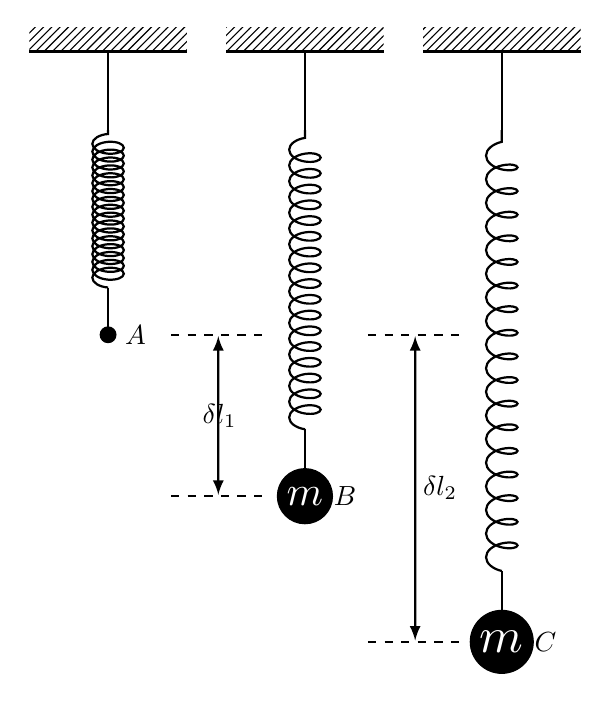
\begin{tikzpicture}[yshift=0cm,every node/.style={draw,outer sep=0pt,thick}]
\begin{scope}[xshift=-2.5cm]
\mola{1mm}{-3cm}{-0.1cm}{0}
\node[draw=none,right=.1cm] at (pt3)(a) {$A$};
\draw [thick,dashed] ($(pt3) + (0.8,0)$) -- +(1.2,0)node[draw=none,inner sep = 0,pos=.5](a1){};
\draw [thick,dashed,] ($(pt3) + (3.3,0)$) -- +(1.2,0)node[draw=none,inner sep = 0,pos=.5](a2){};
\end{scope}
%
\begin{scope}
\mola{2mm}{-4.8cm}{-0.35cm}{1.5}
\node[draw=none,right=.25cm] at (pt3)(b) {$B$};
\draw [thick,dashed] ($(pt3) + (-1.7,0)$) -- +(1.2,0)node[draw=none,inner sep = 0,pos=.5](b1){};
\draw[thick,latex-latex] (a1) -- (b1)node[draw=none,inner sep = 0,pos=.5,right=-0.2cm]{$\delta l_1$};
\end{scope}
%
\begin{scope}[xshift=2.5cm]
\mola{3mm}{-6.6cm}{-0.4cm}{1.8}
\node[draw=none,right=.3cm] at (pt3)(b) {$C$};
\draw [thick,dashed] ($(pt3) + (-1.7,0)$) -- +(1.2,0)node[draw=none,inner sep = 0,pos=.5](c1){};
\draw[thick,latex-latex] (a2) -- (c1)node[draw=none,inner sep = 0,pos=.5,right=0.1cm]{$\delta l_2$};
\end{scope}
%
\end{tikzpicture}
%
\end{document}